\documentclass[../main.tex]{subfiles}
\graphicspath{{\subfix{../images/}}}
\begin{document}

Baseado nos conceitos apresentados, foi projetado, simulado e desenvolvido um robô quadrúpede nomeado de Caramelo (figuras \ref{fig:terrenos}, \ref{fig:caramel_body} e \ref{fig:moving_body}). Caramelo é um robô quadrúpede de pequeno porte voltado para pesquisa e educação. Seu \textit{hardware} foi modelado inteiramente pela equipe e impresso com impressora 3D no material ABS. Os atuadores do robô são servomotores do modelo \textit{dynamixel} MX-28 e sua central de processamento é composta por uma \textit{RaspberryPi} 4. Além disso, ele conta com um sensor inercial modelo MPU6050, que está instalado no corpo do robô. Este sensor contém um giroscópio e um acelerômetro, o que permite obter a aceleração linear, a velocidade angular e a orientação do corpo do robô. Todo o \textit{software} foi desenvolvido com o \textit{Robot Operating System 2 Humble} (\textit{ROS2}) \cite{ROS2Humble}, que consiste em um \textit{framework} de robótica \textit{open source} com vários recursos disponíveis para facilitar o desenvolvimento de sistemas robóticos.

A estrutura do Caramelo é do tipo mamífero e a configuração das pernas é a \textit{full-elbow}. Além disso, possui 3 GDL por perna, o que permite uma grande liberdade de movimentação para as patas. Seu \textit{design} foi pensado para favorecer o balanço de massas entre o corpo e as pernas do robô, ou seja, a maior parte da massa se encontra no corpo ou próxima a ele. Os componentes eletrônicos internos, que abrangem sensores, unidades de processamento e a interface de comunicação com os atuadores, foram dispostos de forma simétrica, a fim de manter o centro de massa o mais próximo do centro do corpo. Os motores (componentes que contribuem com a maior massa para o sistema) foram dispostos o mais próximo possível do corpo. Um destaque para o motor que atua na junta da tíbia, é que foi instalado na parte de cima do fêmur com o objetivo de diminuir o momento de inércia da perna. Essa escolha demandou a adição de um sistema de transmissão entre o eixo do motor e a tíbia, formado por uma haste rígida de metal com duas juntas esféricas nas extremidades.

A locomoção do Caramelo foi desenvolvida baseada nas marchas periódicas e simétricas. Dessa forma, foi adotada a marcha \textit{trot} como a marcha principal do robô. Embora sua estrutura permita a realização de muitos outros tipos de marcha, neste trabalho, foi considerada apenas o \textit{trot}, devido a sua simplicidade e eficiência. Com o objetivo de diminuir a complexidade do controle de locomoção, foi adotada uma marcha descontínua, ou seja, o corpo do robô se desloca apenas quando todas as patas estão do solo. A sequência de etapas da marcha do Caramelo pode ser vista na figura \ref{fig:trot_pattern}, na qual as áreas em branco representam a etapa de \textit{swing} e as em cinza a de \textit{stance}. É possível perceber que sempre o mesmo par de pernas diagonais se move no mesmo instante. Entre duas etapas consecutivas de \textit{swing}, há um momento em que todas as patas estão em \textit{stance}, que é quanto o corpo do robô é deslocado no sentido desejado de locomoção.

\begin{figure}[!htb]
  \centering
  \caption{Padrão de movimentação da marcha para cada perna.}
  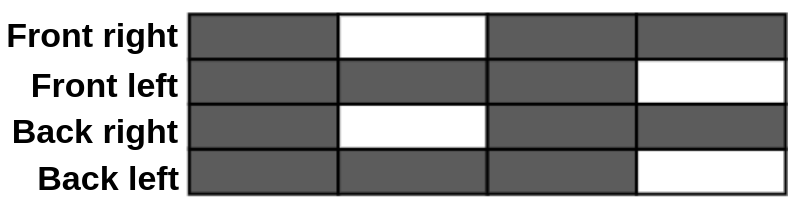
\includegraphics[width=0.45\textwidth]{trot_pattern.png}
  \vfill
  Fonte: autores.
  \vspace{-\baselineskip}
  \label{fig:trot_pattern}
\end{figure}

O sistema de controle do robô é composto por dois subsistemas principais: os controladores individuais de cada junta e os controladores da angulação do corpo do robô. Os controladores das juntas são os próprios controladores PID embarcados nos motores \textit{dynamixel}. Foi utilizada a interface de controle de posição com o atuador, de forma que o \textit{setpoint} de controle enviado para cada motor é o ângulo em radianos para o qual ele deve rotacionar. O modelo cinemático do robô, apresentado na seção \ref{sec:detail_inv_kinematics}, é o responsável por mapear não apenas a posição tridimensional de cada pata com a angulação de cada junta, mas também a posição do corpo em seis dimensões: translação e rotação em $(x, y, z)$. Dessa forma, é possível controlar cada pata e o corpo do robô ao mesmo tempo de forma independente. Os controladores de angulação do corpo são dois controladores PID em paralelo, responsáveis por controlar o ângulo de \textit{pitch} (rotação em $y$) e o de \textit{roll} (rotação em $x$).

O planejador de marchas é o responsável por controlar cada pata do robô e, por consequência, o corpo. Ele calcula a trajetória que cada pata deve realizar, com base nas etapas de \textit{stance} e \textit{swing}, e envia o próximo ponto em que cada pata deve estar a uma frequência de $\SI{50}{\hertz}$. Além disso, ele também considera o esforço de controle enviado pelos controladores de angulação, a fim de manter o corpo do robô em $0^{\circ}$ a todo momento.

A seguir, serão apresentados o desenvolvimento do modelo cinemático, dos controladores de angulação e da trajetória que cada pata realiza na etapa de \textit{swing}.

\subsection{Modelo cinemático do Caramelo}
\label{sec:detail_inv_kinematics}

Como dito anteriormente, o modelo cinemático é utilizado para resolver a cinemática inversa e a cinemática direta do robô. Para a cinemática direta, foi utilizado o pacote \textit{tf2}, um recurso disponível no \textit{ROS2} que facilita o gerenciamento de transformações entre eixos de coordenadas. A cinemática inversa, por outro lado, foi feita com base em uma análise geométrica. As variáveis $\theta_1$, $\theta_2$ e $\theta_3$ expressam a posição angular de cada uma das juntas de uma perna do robô e são calculadas com auxílio das equações \ref{eq:theta1} a \ref{eq:B} em função da posição $(x_{IK}, y_{IK}, z_{IK})$ desejada para a pata e dos comprimentos $L_1$, $L_2$ e $L_3$ (figura \ref{fig:caramel_tfs}).
\begin{equation}
  \label{eq:theta1}
  \theta_1 = \arctan{(\frac{x_{IK}}{y_{IK}})} - \arctan{(\frac{L_1}{a})}
\end{equation}
\begin{equation}
  \label{eq:theta2}
  \theta_2 = \frac{\pi}{2} - \arctan{(\frac{a}{z_{IK}}}) - \arctan{(\frac{\sqrt{1-A^2}}{A})}
\end{equation}
\begin{equation}
  \label{eq:theta3}
  \theta_3 = \arctan(\frac{\sqrt{1-B^2}}{B})
\end{equation}
\begin{equation}
  \label{eq:a}
  a = \sqrt{x_{IK}^2+y_{IK}^2-L_1^2}
\end{equation}
\begin{equation}
  \label{eq:A}
  A =\frac{a^2+z^2+L_2^2-L_3^2}{2L_2\sqrt{a^2+z_{IK}^2}}
\end{equation}
\begin{equation}
  \label{eq:B}
  B = \frac{a^2+z_{IK}^2-L_2^2-L_3^2}{2L_2L_3}
\end{equation}

\begin{figure}[!htb]
  \centering
  \caption{Links da perna do robô.}
  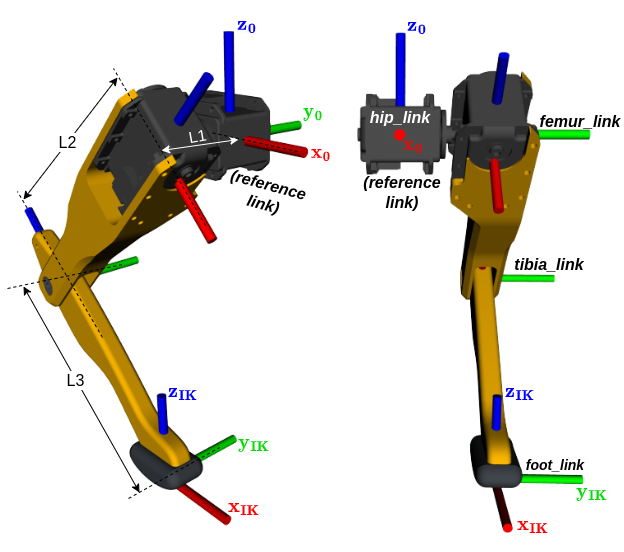
\includegraphics[width=0.4\textwidth]{caramel_tfs.png}
  
  Fonte: autores.
  \label{fig:caramel_tfs}
\end{figure}

Essas equações são úteis para o cálculo da posição de uma única perna, mas são insuficientes para realizar a cinemática do corpo do robô. Desta forma, um \textit{frame} central, chamado de \textit{base\_link} (figura \ref{fig:caramel_body}), é utilizado como referência, e uma matriz $T_M$ (eqs. \ref{eq:Tm} e \ref{eq:Rxyz}) é utilizada para realizar a cinemática do corpo, a partir das translações $(x_c, y_c, z_c)$ e rotações $(\alpha, \beta, \gamma)$ desejadas, sendo possível controlar cada um dos 6 graus de liberdade. Para isso, as transformações $T_{FR}$, $T_{FL}$, $T_{BL}$ e $T_{BR}$ de cada um dos ombros (\textit{hip\_links}) em relação ao \textit{base\_link} são necessárias.
\begin{equation}
  \label{eq:Tm}
  T_M =
  \begin{bmatrix}
      &         &   & x_c \\
      & R_{xyz} &   & y_c \\
      &         &   & z_c \\
    0 & 0       & 0 & 1
  \end{bmatrix}
\end{equation}
\begin{equation}
  \label{eq:Rxyz}
  \begin{split}
    R_{xyz} =
    \begin{bmatrix}
      1 & 0          & 0           \\
      0 & \cos\alpha & -\sin\alpha \\
      0 & \sin\alpha & \cos\alpha
    \end{bmatrix}
    \\.
    \begin{bmatrix}
      \cos\beta  & 0 & \sin\beta \\
      0          & 1 & 0         \\
      -\sin\beta & 0 & \cos\beta
    \end{bmatrix}
    \\.
    \begin{bmatrix}
      \cos\gamma & -\sin\gamma & 0 \\
      \sin\gamma & \cos\gamma  & 0 \\
      0          & 0           & 1
    \end{bmatrix}
  \end{split}
\end{equation}

\begin{figure}[!htb]
  \centering
  \caption{Eixos do robô em posição de repouso.}
  \vspace{-0.75cm}
  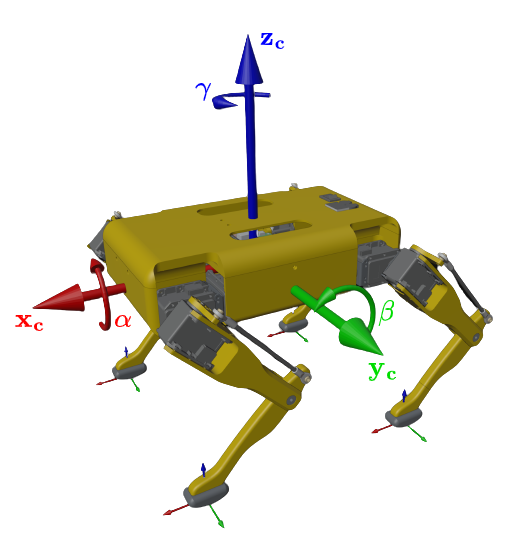
\includegraphics[width=0.35\textwidth]{caramel_body.drawio.png}
  
  Fonte: autores.
  \label{fig:caramel_body}
\end{figure}

O cálculo das angulações de cada perna então é feito utilizando como entrada os valores $(x_{IK}, y_{IK}, z_{IK})$ resultantes de cada uma das transformações, conforme a equação \ref{eq:xyzik}. O mesmo cálculo é feito para as demais pernas, utilizando  $T_{FL}$, $T_{BL}$ e $T_{BR}$.
\begin{equation}
  \label{eq:xyzik}
  \begin{bmatrix}
    x_{IK} \\
    y_{IK} \\
    z_{IK} \\
    1
  \end{bmatrix}= (T_M.T_{FR})^{-1}.
  \begin{bmatrix}
    x \\
    y \\
    z \\
    1
  \end{bmatrix}
\end{equation}

Desta forma, a Cinemática Inversa é capaz de computar as angulações  $\theta_1$, $\theta_2$ e $\theta_3$ de cada uma das pernas a partir da posição $(x, y, z)$ das patas em relação ao link central do robô e às translações $(x_c, y_c, z_c)$ e rotações $(\alpha, \beta, \gamma)$ desejadas para o corpo. Entretanto, em muitos casos é mais conveniente realizar o cálculo dos ângulos passando como entrada as posições $(x, y, z)$ das patas em relação à sua posição \textit{default}, ou seja, a posição do seu \textit{foot\_link} quando o robô está em seu estado de repouso (figura \ref{fig:caramel_body}). Para isso, é possível realizar, previamente ao cálculo das angulações, mais uma transformação, desta vez do \textit{base\_link} para cada uma das posições \textit{default} das patas (equação \ref{eq:xyzik_foot}).
\begin{equation}
  \label{eq:xyzik_foot}
  \begin{bmatrix}
    x_{ik} \\
    y_{ik} \\
    z_{ik} \\
    1
  \end{bmatrix}= (T_M.T_{FR})^{-1}.
  (F_{FR}.
  \begin{bmatrix}
    x \\
    y \\
    z \\
    1
  \end{bmatrix})
\end{equation}

\subsection{Controle de angulação}

Os controladores de angulação são dois controladores PID iguais em paralelo responsáveis por controlar a rotação de \textit{roll} e \textit{pitch} do corpo do robô. Eles atuam de forma independente, controlando a rotação do corpo em ambos os eixos simultaneamente. 
% \begin{figure}[!htb]
%   \centering
%   \caption{Controlador PID projetado.}
%   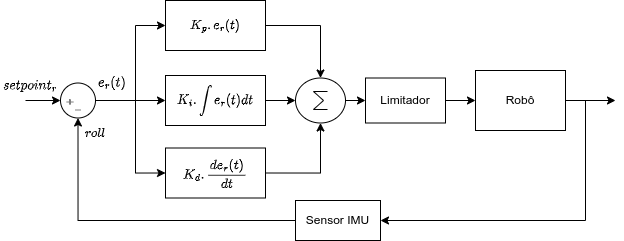
\includegraphics[width=0.48\textwidth]{PID.drawio.png}
%   Fonte: autores.
%   \label{fig:pid}
%   \vspace{-\baselineskip}
% \end{figure}
O IMU é o sensor responsável por medir a rotação do corpo do robô, possibilitando a realimentação das saídas do sistema. Existe um limitador na saída do controlador para evitar que sejam enviados valores que extrapolem os limites de rotação das juntas do robô. Os esforços de controle são enviados para o planejador de marchas que, por sua vez, envia os comandos de movimentação para os controladores das juntas.

\subsection{Planejador de trajetória}

O planejador de trajetória é responsável por calcular a trajetória que cada pata deve realizar, tanto na fase de \textit{stance} quanto na fase de \textit{swing}. Para o Caramelo, a trajetória é uma curva cicloidal em ambas as etapas. Como apresentado em \cite{Shi2021}, uma curva cicloidal pode ser definida no espaço tridimensional entre os pontos $(x_o, y_o, z_o)$ e $(x_f, y_f, z_f)$ em função do tempo $t$ pelas equações (\ref{eq:traj_x}) a (\ref{eq:traj_k}), sendo $H$ a altura do passo e $T$ o período.
\begin{equation}
  x = (x_f - x_o) \frac{K - \sin{(K)}}{2 \pi} + x_o
  \label{eq:traj_x}
\end{equation}
\begin{equation}
  y = (y_f - y_o) \frac{K - \sin{(K)}}{2 \pi} + y_o
  \label{eq:traj_y}
\end{equation}
\begin{equation}
  z = H \frac{1 - \cos{(K)}}{2} + z_o
  \label{eq:traj_z}
\end{equation}
\begin{equation}
  K = \frac{2 \pi t}{T}
  \label{eq:traj_k}
\end{equation}

O gráfico de uma curva cicloidal no espaço 3D pode ser vista na figura \ref{fig:traj_space}. A mesma trajetória é ilustrada na figura \ref{fig:traj_time} em função do tempo. É possível perceber que a curva possui primeira derivada nula no momento em que a pata toca o solo, o que é favorável ao controle de malha aberta já que quanto mais suave for a aterrissagem, menos distúrbios são causados no sistema.
\begin{figure*}[h]
  \centering
  \caption{Trajetórias cicloidais para o passo de robô.}
  \begin{subfigure}[t]{0.32\textwidth}
    \centering
    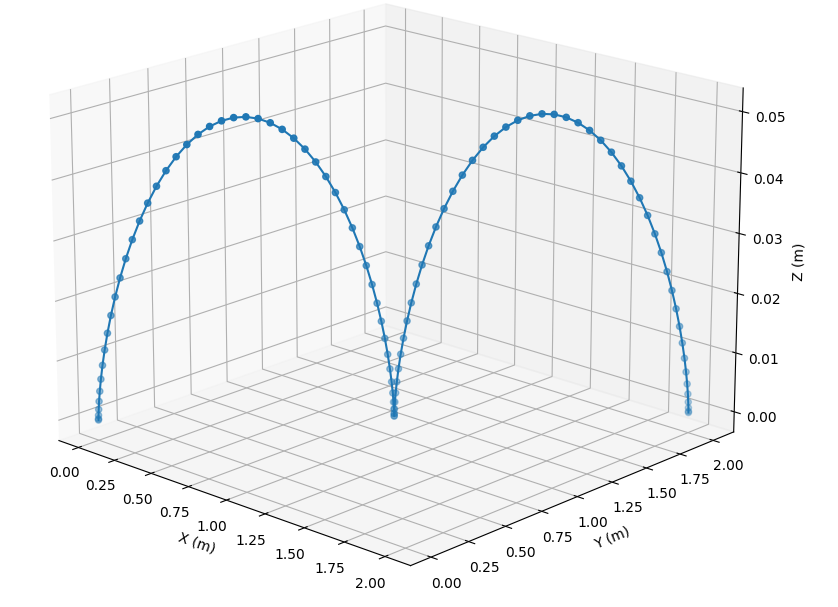
\includegraphics[width=1.0\textwidth]{Cycloid_space.png}
    \caption{Curva no espaço 3D.}
    \label{fig:traj_space}
  \end{subfigure}
  \begin{subfigure}[t]{0.32\textwidth}
    \centering
    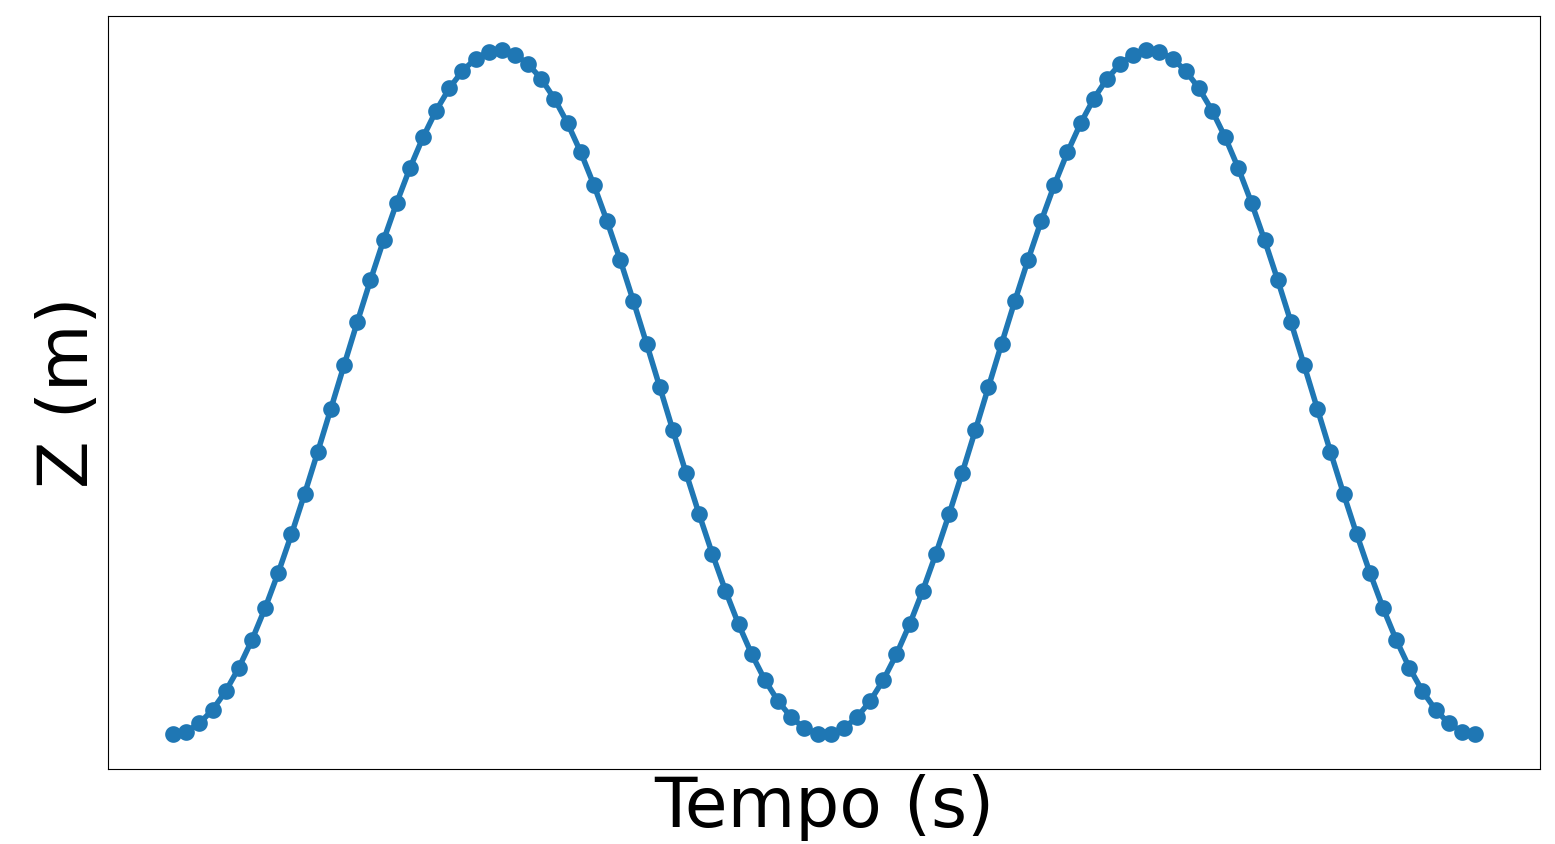
\includegraphics[width=1.0\textwidth]{Cycloid_time.png}
    \caption{Curva no tempo.}
    \label{fig:traj_time}
  \end{subfigure}
  \begin{subfigure}[t]{0.32\textwidth}
    \centering
    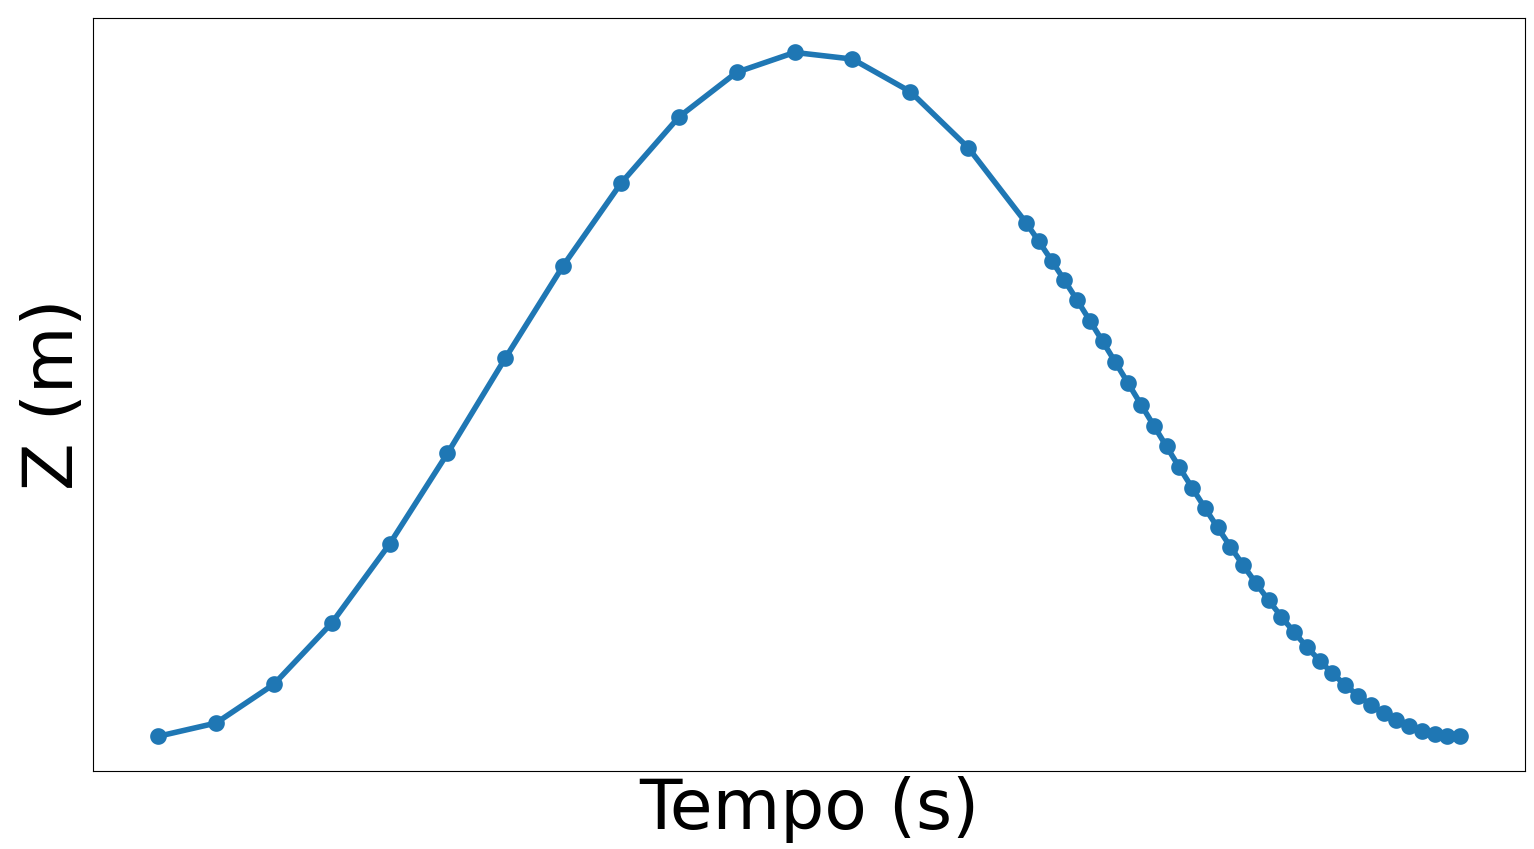
\includegraphics[width=1.0\textwidth]{Cycloid_modified.png}
    \caption{Curva com disposição de pontos modificada.}
    \label{fig:traj_time_modified}
  \end{subfigure}
  \vfill
  Fonte: autores.
  \vspace{-\baselineskip}
  \label{fig:traj_curve}
\end{figure*}

Além da altura, distâncias em $x$ e $y$ e período, o planejador de trajetória do Caramelo também conta com dois parâmetros que têm como objetivo melhorar ainda mais o controle da força com que a pata toca o chão. Como os atuadores do robô são servomotores controlados por posição, o torque é proporcional ao deslocamento que este deve realizar entre os pontos da trajetória. Ou seja, quanto maior a resolução da trajetória, mais suave será o movimento. No entanto, a resolução da trajetória $N$ é fixa, data em função do período do passo e da frequência de controle do planejador de marchas ($\SI{50}{\hertz}$) $N = 50T$. Logo, a estratégia adotada é a de espaçar a mesma quantidade de pontos de forma desigual ao longo do período do passo, de forma que haja mais pontos próximos ao momento em que a pata aterrissa no solo e menos pontos próximos ao momento em que ele é erguido. O parâmetro $P_T$ é uma fração do período total do passo e o parâmetro $P_N$ a fração do número total de pontos do passo que deve se encontrar entre o tempo $0$ e $P_T \cdot T$. Em outras palavras, se $P_T = 0,66$ e $P_N = 0,33$, $33\%$ de $N$ estará nos primeiro dois terços do período, enquanto os $67\%$ restantes estarão no um terço final. A trajetória considerando esses parâmetros está ilustrada na figura \ref{fig:traj_time_modified}.

\end{document}
